% Options for packages loaded elsewhere
\PassOptionsToPackage{unicode}{hyperref}
\PassOptionsToPackage{hyphens}{url}
%
\documentclass[
  english,
  man]{apa6}
\author{\phantom{0}}
\date{}

\usepackage{amsmath,amssymb}
\usepackage{lmodern}
\usepackage{iftex}
\ifPDFTeX
  \usepackage[T1]{fontenc}
  \usepackage[utf8]{inputenc}
  \usepackage{textcomp} % provide euro and other symbols
\else % if luatex or xetex
  \usepackage{unicode-math}
  \defaultfontfeatures{Scale=MatchLowercase}
  \defaultfontfeatures[\rmfamily]{Ligatures=TeX,Scale=1}
\fi
% Use upquote if available, for straight quotes in verbatim environments
\IfFileExists{upquote.sty}{\usepackage{upquote}}{}
\IfFileExists{microtype.sty}{% use microtype if available
  \usepackage[]{microtype}
  \UseMicrotypeSet[protrusion]{basicmath} % disable protrusion for tt fonts
}{}
\makeatletter
\@ifundefined{KOMAClassName}{% if non-KOMA class
  \IfFileExists{parskip.sty}{%
    \usepackage{parskip}
  }{% else
    \setlength{\parindent}{0pt}
    \setlength{\parskip}{6pt plus 2pt minus 1pt}}
}{% if KOMA class
  \KOMAoptions{parskip=half}}
\makeatother
\usepackage{xcolor}
\IfFileExists{xurl.sty}{\usepackage{xurl}}{} % add URL line breaks if available
\IfFileExists{bookmark.sty}{\usepackage{bookmark}}{\usepackage{hyperref}}
\hypersetup{
  pdflang={en-EN},
  hidelinks,
  pdfcreator={LaTeX via pandoc}}
\urlstyle{same} % disable monospaced font for URLs
\usepackage{graphicx}
\makeatletter
\def\maxwidth{\ifdim\Gin@nat@width>\linewidth\linewidth\else\Gin@nat@width\fi}
\def\maxheight{\ifdim\Gin@nat@height>\textheight\textheight\else\Gin@nat@height\fi}
\makeatother
% Scale images if necessary, so that they will not overflow the page
% margins by default, and it is still possible to overwrite the defaults
% using explicit options in \includegraphics[width, height, ...]{}
\setkeys{Gin}{width=\maxwidth,height=\maxheight,keepaspectratio}
% Set default figure placement to htbp
\makeatletter
\def\fps@figure{htbp}
\makeatother
\setlength{\emergencystretch}{3em} % prevent overfull lines
\providecommand{\tightlist}{%
  \setlength{\itemsep}{0pt}\setlength{\parskip}{0pt}}
\setcounter{secnumdepth}{-\maxdimen} % remove section numbering
% Make \paragraph and \subparagraph free-standing
\ifx\paragraph\undefined\else
  \let\oldparagraph\paragraph
  \renewcommand{\paragraph}[1]{\oldparagraph{#1}\mbox{}}
\fi
\ifx\subparagraph\undefined\else
  \let\oldsubparagraph\subparagraph
  \renewcommand{\subparagraph}[1]{\oldsubparagraph{#1}\mbox{}}
\fi
% Manuscript styling
\usepackage{upgreek}
\captionsetup{font=singlespacing,justification=justified}

% Table formatting
\usepackage{longtable}
\usepackage{lscape}
% \usepackage[counterclockwise]{rotating}   % Landscape page setup for large tables
\usepackage{multirow}		% Table styling
\usepackage{tabularx}		% Control Column width
\usepackage[flushleft]{threeparttable}	% Allows for three part tables with a specified notes section
\usepackage{threeparttablex}            % Lets threeparttable work with longtable

% Create new environments so endfloat can handle them
% \newenvironment{ltable}
%   {\begin{landscape}\centering\begin{threeparttable}}
%   {\end{threeparttable}\end{landscape}}
\newenvironment{lltable}{\begin{landscape}\centering\begin{ThreePartTable}}{\end{ThreePartTable}\end{landscape}}

% Enables adjusting longtable caption width to table width
% Solution found at http://golatex.de/longtable-mit-caption-so-breit-wie-die-tabelle-t15767.html
\makeatletter
\newcommand\LastLTentrywidth{1em}
\newlength\longtablewidth
\setlength{\longtablewidth}{1in}
\newcommand{\getlongtablewidth}{\begingroup \ifcsname LT@\roman{LT@tables}\endcsname \global\longtablewidth=0pt \renewcommand{\LT@entry}[2]{\global\advance\longtablewidth by ##2\relax\gdef\LastLTentrywidth{##2}}\@nameuse{LT@\roman{LT@tables}} \fi \endgroup}

% \setlength{\parindent}{0.5in}
% \setlength{\parskip}{0pt plus 0pt minus 0pt}

% \usepackage{etoolbox}
\makeatletter
\patchcmd{\HyOrg@maketitle}
  {\section{\normalfont\normalsize\abstractname}}
  {\section*{\normalfont\normalsize\abstractname}}
  {}{\typeout{Failed to patch abstract.}}
\patchcmd{\HyOrg@maketitle}
  {\section{\protect\normalfont{\@title}}}
  {\section*{\protect\normalfont{\@title}}}
  {}{\typeout{Failed to patch title.}}
\makeatother
\shorttitle{SHORTTITLE}
\usepackage{csquotes}
\usepackage{float}
\usepackage{sectsty}
\ifXeTeX
  % Load polyglossia as late as possible: uses bidi with RTL langages (e.g. Hebrew, Arabic)
  \usepackage{polyglossia}
  \setmainlanguage[]{english}
\else
  \usepackage[main=english]{babel}
% get rid of language-specific shorthands (see #6817):
\let\LanguageShortHands\languageshorthands
\def\languageshorthands#1{}
\fi
\ifLuaTeX
  \usepackage{selnolig}  % disable illegal ligatures
\fi


\affiliation{\phantom{0}}

\begin{document}

\hypertarget{chapitre-2-utiliser-le-test-bf-emph-t-de-welch}{%
\section{\texorpdfstring{Chapitre 2 : Utiliser le test \(\bf \emph t\) de Welch}{Chapitre 2 : Utiliser le test \textbackslash bf \textbackslash emph t de Welch}}\label{chapitre-2-utiliser-le-test-bf-emph-t-de-welch}}

\begin{figure}

{\centering 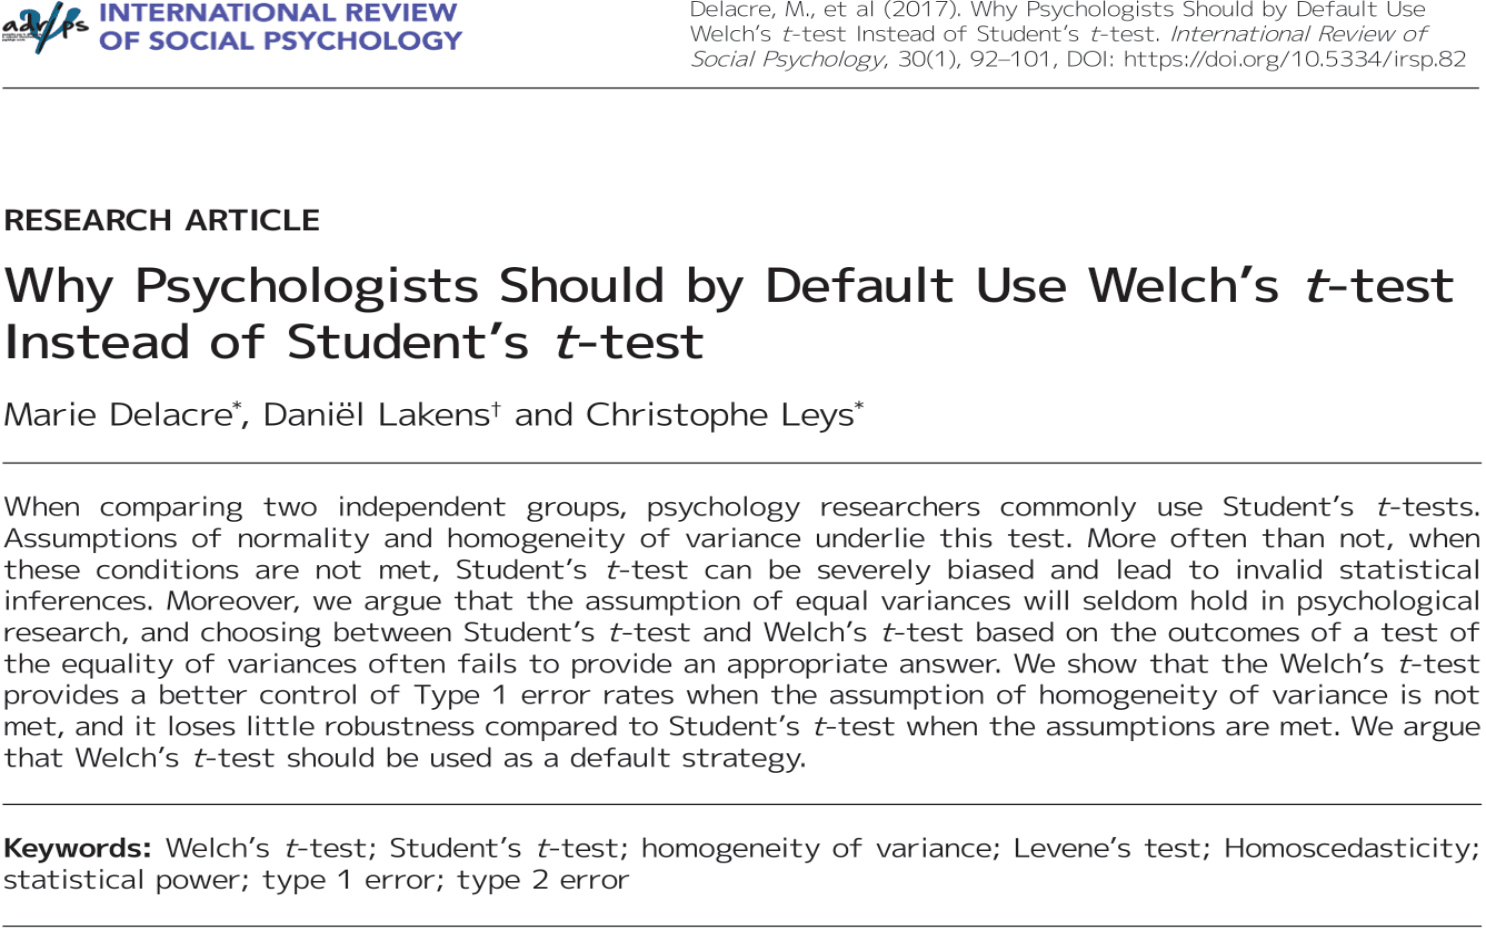
\includegraphics[height=0.45\textheight]{C:/Users/mdelacre/Documents/Github project/thesis/Chapitre 2/Chapitre 2-couverture} 

}

\caption{ }\label{fig:chp2p1}
\end{figure}

Independent samples \(t\)-tests are commonly used in the psychological literature to statistically test differences between means. There are different types of \(t\)-tests, such as Student's \(t\)-test, Welch's \(t\)-test, Yuen's \(t\)-test, and a bootstrapped \(t\)-test. These variations differ in the underlying assumptions about whether data is normally distributed, and whether variances in both groups are equal (see e.g., Rasch et al., 2011; Yuen, 1974). Student's \(t\)-test is the default method to compare two groups in psychology. The alternatives that are available are considerably less often reported. This is surprising, since Welch's \(t\)-test is often the preferred choice, and is available in practically all statistical software packages.

In this article, we will review the differences between Welch's \(t\)-test and Student's \(t\)-test, and suggest that Welch's \(t\)-test is a better default for the social sciences than Student's \(t\)-test. \color{red}We do not include the bootstrapped \(t\)-test because it is known to fail in specific situations, such as when there are unequal sample sizes and standard deviations differ moderately (\textbf{hayes\_further\_2007?}).
\color{black}
When performing a \(t\)-test, several software packages (i.e., R and Minitab) present Welch's \(t\)-test by default. Users can request Student's \(t\)-test, but only after explicitly stating that the assumption of equal variances is met. Student's \(t\)-test is a parametric test, which means it relies on assumptions about the data that are analyzed. Parametric tests are believed to be more powerful than non-parametric tests (i.e.~tests that do not require assumptions about the population parameters, \textbf{sheskin\_handbook\_2003?}). However, Student's \(t\)-test is generally only more powerful if the data are normally distributed (the assumption of normality) and the variances are equal in both groups (homoscedasticity, the assumption of homogeneity of variance; Carroll \(\&\) Schneider,
1985; Erceg-Hurn \(\&\) Mirosevich, 2008).

When sample sizes are equal between groups, Student's \(t\)-test is robust to violations of the assumption of equal variances as long as sample sizes are big enough to allow correct estimates of both means and standard deviations (i.e.~\(n \ge 5\))\footnote{There is a Type I error rate inflation in a few cases where sample sizes are extremely small and SDR is big (for example, when \(n_1 = n_2 = 3\) are sampled from uniform distributions and SDR = 2, the Type I error rate = 0.083; or when \(n_1 = 3\) is sampled from a uniform distribution and \(n_2 = 3\) is sampled from a double exponential distribution). However, with extremely small sample sizes (\(n_1+n_2 \le 5\)), the estimate of means and standard deviations is extremely inaccurate anyway. As we mentioned in Table A2 (see the additional file), the smaller the sample size, the further the average standard deviation is from the population standard deviation, and the larger the dispersion around this average.}, except when distributions underlying the data have very high skewness and kurtosis, such as a chi-square distribution with 2 degrees of freedom. However, if variances are \emph{not} equal across groups, and the sample sizes differ across independent groups, Student's \(t\)-test can be severely biased, and lead to invalid statistical inferences (\textbf{erceg-hurn\_modern\_2008?}).\footnote{This is called the Behren-Fisher problem  (Hayes $\&$ Cai, 2007).}\footnote{In a simulation that explored Type 1 error rates, we varied the size of the first sample from 10 to 40 in steps of 10, and the sample sizes ratio and the standard deviation ratio from 0.5 to 2 in steps of 0.5, resulting in 64 simulations designs. Each design was tested 1,000,000 times. Considering these parameter values, we found that the alpha level can be inflated up to .11 or deflated down to .02 (See the Additional file).} Here, we argue that there are no strong reasons to assume equal variances in the psychological literature by default nor substantial costs in abandoning this assumption.

In this article, we will first discuss why we need a default test and why a two-step procedure where researchers decide whether or not to use Welch's \(t\)-test based on a check of the assumption of normality and equal variances is undesirable. Then, we will discuss whether the assumption of equal variances is plausible in psychology and point out research areas where this assumption is implausible. We will then review differences between Student's \(t\)-test and Welch's \(t\)-test and show through simulations that the bias in Type I error rates when Student's \(t\)-test is used has a larger impact on statistical inferences than the rather modest impact on the Type II error rate of always using Welch's \(t\)-test by default. Given our analysis, and the availability of Welch's \(t\)-test in all statistical software, we recommend a procedure where Welch's \(t\)-test is used when sample sizes are unequal.

\hypertarget{limitations-of-two-step-procedures}{%
\subsection{Limitations of Two-Step Procedures}\label{limitations-of-two-step-procedures}}

Readers may have learned that the assumptions of normality and of equal variances (or the homoscedasticity assumption) must be examined using assumption checks prior to performing any \(t\)-test. When data are not normally distributed, with small sample sizes, alternatives should be used. Classic nonparametric statistics are well known, such as the Mann-Whitney \(U\)-test and Kruskal-Wallis. However, unlike a \(t\)-test, tests based on rank assume that the distributions are the same between groups. Any departure to this assumption, such as unequal variances, will therefore lead to the rejection of the assumption of equal distributions (\textbf{zimmerman\_statistical\_2000?}). Alternatives exist, known as the ``modern robust statistics'' (\textbf{wilcox\_modern\_2013?}). For example, data sets with low kurtosis (i.e., a distribution flatter than the normal distribution) should be analyzed with the two-sample trimmed \(t\)-test for unequal population variances, also called Yuen's \(t\)-test (\textbf{luh\_approximate\_2007?}; \textbf{yuen\_two-sample\_1974?}). Yuen's \(t\)-test, also called ``20\(\%\) trimmed means test,'' is an extension of the Welch's \(t\)-test and is allegedly more robust in case of non-normal distributions (\textbf{wilcox\_modern\_2003?}). Yuen's \(t\)-test consists of removing the lowest and highest 20 percent of the data and applying Welch's \(t\)-test on the remaining values. The procedure is explained and well-illustrated in a paper by Erceg-Hurn and Mirosevich (2008).

With respect to the assumption of homogeneity of variance, if the test of the equality of variance is non-significant, and the assumption of equal variances cannot be rejected, homoscedastic methods such as the Student's \(t\)-test should be used (Wilcox et al., 2013). If the test of the equality of variances is significant, Welch's \(t\)-test should be used instead of Student's \(t\)-test, because the assumption of equal variances is violated. However, testing the equality of variances before deciding which \(t\)-test is performed is problematic for several reasons, which will be explained after having described some of the most widely used tests of equality of variances.

\hypertarget{different-ways-to-test-for-equal-variances}{%
\subsection{Different ways to test for equal variances}\label{different-ways-to-test-for-equal-variances}}

Researchers have proposed several tests for the assumption of equal variances. Levene's test and the \(F\)-ratio test are the most likely to be used by researchers because they are available in popular statistical software (\textbf{hayes\_further\_2007?}). Levene's test is the default option in SPSS. Levene's test is the One-Way ANOVA computed on the terms \(|X_{ij}-\hat{\theta_j}|\), where \(X_{ij}\) is the \(i^{th}\) observation in the \(j^{th}\) group, and \(\hat{\theta_j}\) is the ``center'' of the distribution for the \(j^{th}\) group (\(j=1,2\), \textbf{carroll\_note\_1985?}). In R, the ``center'' is by default the median, which is also called ``Brown Forsythe test for equal variances.'' In SPSS, the ``center'' is by default the mean (which is the most powerful choice when the underlying data are symmetrical).\footnote{ Other variants have been proposed such as the 20 percent trimmed mean (\textbf{lim\_comparison\_1996?}).} The \(F\)-ratio statistic is obtained by computing \(\frac{max(S_1,S_2)}{min(S_1,S_2)}\) where \(S_j\) is the sample standard deviation of the \(j^{th}\) group (\(j=1,2\)). A generalization of the \(F\)-ratio test, to be used when there are more than two groups to compare, is known as the Bartlett's test.

The \(F\)-ratio test and the Bartlett test are powerful, but they are only valid under the assumption of normality and collapse as soon as one deviates even slightly from the normal distribution. They are therefore not recommended (\textbf{rakotomalala\_comparaison\_2008?}).

Levene's test is more robust than Bartlett's test and the \(F\)-ratio test, but there are three arguments against the use of Levene's test. First, there are several ways to compute Levene's test (i.e., using the median or mean as center), and the best version of the test for equal variances depends on how symmetrically the data is distributed, which is itself difficult to statistically quantify.

Second, performing two tests (Levene's test followed by a \(t\)-test) on the same data makes the alpha level and power of the \(t\)-test dependent upon the outcome of Levene's test. When we perform Student's or Welch's \(t\)-test conditionally on a significant Levene's test, the long-run Type I and Type II error rates will depend on the power of Levene's test. When the power of Levene's test is low, the error rates of the conditional choice will be very close to Student's error rates (because the probability of choosing Student's \(t\)-test is very high). On the other hand, when the power of Levene's test is very high, the error rates of the conditional choice will be very close to Welch's error rate (because the probability of choosing Welch's \(t\)-test is very high; see \textbf{rasch\_two-sample\_2011?}). When the power of Levene's test is medium, the error rates of the conditional choice will be somewhere between Student's and Welch's error rates (see, e.g., \textbf{zimmerman\_note\_2004?}). This is problematic when the test most often performed actually has incorrect error rates.

Third, and relatedly, Levene's test can have very low power, which leads to Type II errors when sample sizes are small and unequal (\textbf{nordstokke\_cautionary\_2007?}). As an illustration, to estimate the power of Levene's test, we simulated 1,000,000 simulations with balanced designs of different sample sizes (ranging from 10 to 80 in each condition, with a step of 5) under three population standard deviation ratio (SDR = \(\frac{\sigma_2}{\sigma_1}\) where \(\sigma_j\) is the population standard deviation of the \(j^{th}\) group; \(j=1,2\)) : respectively 1.1, 1.5 and 2, yielding 45,000,000 simulations in total. When SDR = 1, the equal variances assumption is true, when SDR \textgreater{} 1 the standard deviation of the second population is bigger than the standard deviation of the first population, and when SDR \textless{} 1 the standard deviation of the second population is smaller than the standard deviation of the first population. We ran Levene's test centered around the mean and Levene's test centered around the median and estimated the power (in \(\%\)) to detect unequal variances, with equal sample sizes (giving the best achievable power for a given total \(n_1+n_2=N\); see Figure \ref{fig:chp2fig1}).\footnote{Because sample sizes are equal for each pair of samples, which sample has the bigger standard deviation is not applicable. In this way, $SDR = X$ will return the same answer in terms of $\%$ power of Levene’s test as $SDR = \frac{1}{X}$. For example, SDR = 2 will return the same answer as SDR = 0.5.}

\begin{figure}

{\centering \includegraphics[width=1\linewidth]{C:/Users/mdelacre/Documents/Github project/studentbackup/scripts outputs/Figures/Figure 1/Figure1} 

}

\caption{Estimated power of Levene's test as a function of sample size, SDR and centering parameter}\label{fig:chp2fig1}
\end{figure}

As we can see in the graph in Figure \ref{fig:chp2fig1}, the further SDR is from 1, the smaller the sample size needed to detect a statistically significant difference in the SDR. Furthermore, for each SDR, power curves of the Levene's test based on the mean are slightly above power curves of the Levene's test based on the median, meaning that it leads to slightly higher power than Levene's test based on the median. This can be due to the fact that data is extracted from normal distributions. With asymmetric data, the median would perform better. When SDR = 2, approximately 50 subjects are needed to have 80 percent power to detect differences while approximately 70 subjects are needed to have 95 percent power to detect differences (for both versions of Levene's test). To detect an SDR of 1.5 with Levene's test, approximately 120 subjects are needed to reach a power of 80\(\%\) and about 160 to reach a power of 95\(\%\). Since such an SDR is already very problematic in terms of the type I error rate for the Student's \(t\)-test (\textbf{bradley\_robustness\_1978?}), needing such a large sample size to detect it is a serious hurdle. This issue becomes even worse for lower SDR, since an SDR as small as 1.1 already calls for the use of Welch's \(t\)-test (See Table A3.1 to A3.9 in the additional file). Detecting such a small SDR calls for a huge sample size (a sample size of 160 provides a power rate of 16\(\%\)).

Since Welch's \(t\)-test has practically the same power as Student's \(t\)-test, even when SDR = 1, as explained using simulations later, we should seriously consider using Welch's \(t\)-test by default.

The problems in using a two-step procedure (first testing for equality of variances, then deciding upon which test to use) have already been discussed in the field of statistics (see e.g., Rasch et al., 2011; Ruxton, 2006; Wilcox et al., 2013; Zimmerman,2004), but these insights have not changed the current practices in psychology, as of yet. More importantly, researchers do not even seem to take the assumptions of Student's \(t\)-test into consideration before performing the test, or at least rarely discuss assumption checks. We surveyed statistical tests reported in the journal SPPS (Social Psychological and Personality Science) between April 2015 and April 2016. From the total of 282 studies, 97 used a \(t\)-test (34.4\(\%\)), and the homogeneity of variance was explicitly discussed in only 2 of them. Moreover, based on the reported degrees of freedom in the results section, it seems that Student's \(t\)-test is used most often and that alternatives are considerably less popular. For 7 studies, there were decimals in the values of the degrees of freedom, which suggests Welch's \(t\)-test might have been used, although the use of Welch's \(t\)-test might be higher but not identifiable, because some statisticians recommend to round the degrees of freedom to round numbers.

To explain this lack of attention to assumption checks, some authors have argued that researchers might have a lack of knowledge (or a misunderstanding) of the parametric assumptions and consequences of their violations or that they might not know how to check assumptions or what to do when assumptions are violated (\textbf{hoekstra\_are\_2012?}).\footnote{ For example, many statistical users believe that the Mann-Whitney non-parametric test can cope with both normality and homosedasticity issues (\textbf{ruxton\_unequal\_2006?}). This assumption is false, since the Mann-Whitney test remains sensitive to heterosedasticity (\textbf{grissom\_heterogeneity\_2000?}; \textbf{nachar\_mann-whitney\_2008?}; \textbf{neuhauser\_distribution-free\_2009?}) .} Finally, many researchers don't even know there are options other than the Student's \(t\)-test for comparing two groups (\textbf{erceg-hurn\_modern\_2008?}). How problematic this is depends on how plausible the assumption of equal variances is in psychological research. We will discuss circumstances under which the equality of variances assumption is especially improbable, and provide real-life examples where the assumption of equal variances is violated.

\hypertarget{homogeneity-of-variance-assumptions}{%
\subsection{Homogeneity of Variance Assumptions}\label{homogeneity-of-variance-assumptions}}

The homogeneity of variances assumption is rarely true in real life and cannot be taken for granted when performing a statistical test (\textbf{erceg-hurn\_modern\_2008?}; \textbf{zumbo\_investigation\_1997?}). Many authors have examined real data and noted that SDR is often different from the 1:1 ratio (see, e.g., Grissom, 2000; Erceg-Hurn \(\&\) Mirosevich, 2008). This shows that the presence of unequal variances is a realistic assumption in psychological research.\footnote{Like Bryk and Raudenbush (1988), we note that unequal variances between groups does not systematically mean that population variances are different : standard deviation ratios are more or less biased estimates of population variance (see Table A2 in the additional file). Differences can be a consequence of bias in measurement, such as response styles (\textbf{baumgartner\_response\_2001?}). However, there is no way to determine what part of the variability is due to error rather than the true population value.} We will discuss three origins of unequal standard deviations across two groups of observations : the variability inherent to the use of measured variables, the variability induced by quasi-experimental treatments on measured variables, and the variability induced by different experimental treatments on randomly assigned subjects.

First, psychologists often use \emph{measured variables} (such as age, gender, educational level, ethnic origin, depression level, etc.) instead of random assignment to condition. In their review of comparing psychological findings from all fields of the behavioral sciences across cultures, (\textbf{henrich\_most\_2010?}) suggest that parameters vary largely from one population to another. In other words, variance is not systematically the same in every pre-existing group. For example, (\textbf{feingold\_sex\_1992?}) has shown that intellectual abilities of males were more variable than intellectual abilities of females when looking at several standardized test batteries measuring general knowledge, mechanical reasoning, spatial visualization, quantitative ability, and spelling. Indeed, the variability hypothesis (that men demonstrate greater variability than women) is more than a century old (for a review, see \textbf{shields\_functionalism\_1975?}). In many research domains, such as mathematics performance, there are strong indicators that variances ratios differ between 1.1 and 1.2, although variances ratios do not differ in all countries, and the causes for these differences are not yet clear. Nevertheless, it is an empirical fact that variances ratios can differ among pre-existing groups. Furthermore, some pre-existing groups have different variability by definition. An example from the field of education is the comparison of selective school systems (where students are accepted on basis of selection criterions) versus comprehensive school systems (where all students are accepted whatever their aptitudes; see, e.g., \textbf{hanushek\_does\_2006?}). At the moment that a school accepts its students, variability in terms of aptitude will be greater in a comprehensive school than in a selective school, by definition.

Second, a quasi-experimental treatment can have a different impact on variances between groups. Hanushek and Wößmann (2006) suggest that there is an impact of the educational system on variability in achievement. Even if variability, in terms of aptitude, is greater in a comprehensive school than in a selective school at first, a selective school system at primary school increases inequality (and then variability) in achievement in secondary school. Another example is variability in moods. (\textbf{cowdry\_mood\_1991?}) noted than intra-individual variability is larger in patients suffering of premenstrual syndrome (PMS) than in normal patients, and larger in normal patients than in depressive patients. Researchers studying the impact of an experimental treatment on mood changes can expect a bigger variability of mood changes in patients with PMS than in normal or depressive patients, and thus a higher standard deviation in mood measurements.

Third, while variances of two groups are the same when group assignment is completely randomized, deviation from equality of variances can occur later, as a \emph{consequence of an experimental treatment} (\textbf{cumming\_understanding\_2013?}; \textbf{erceg-hurn\_modern\_2008?}; \textbf{Keppel\_1991?}). For example, psychotherapy for depression can increase the variability in depressive symptoms, in comparison with a control group, because the effectiveness of the therapy will depend on individual differences (\textbf{bryk\_heterogeneity\_1988?}; \textbf{erceg-hurn\_modern\_2008?}). Similarly, (\textbf{kester\_communication\_1969?}) compared the IQ of students from a control group with the IQ of students when high expectancies about students were induced in the teacher. While no effect of teacher expectancy on IQ was found, the variance was bigger in the treatment group than in the control group (56.52 vs.~32.59, that is, SDR \(\approx\) 1.32). As proposed by (\textbf{bryk\_heterogeneity\_1988?}), this can result from the interaction between the treatment and the students' reactions : students can react differently to the induced expectations. More generally, whenever a manipulation has individual moderators, variability should increase compared to a control condition.

Knowing whether standard deviations differ across conditions is important information, but in many fields, we have no accurate estimates of the standard deviation in the population. Whereas we collect population effect sizes in meta-analyses, these meta-analyses often do not include the standard deviations from the literature. As a consequence, we regrettably do not have easy access to aggregated information about standard deviations across research areas, despite the importance of this information. It would be useful if meta-analysts start to code information about standard deviations when performing meta-analyses (\textbf{lakens\_reproducibility\_2016?}), such that we can accurately quantify whether standard deviations differ between groups, and how large the SDR is.

\hypertarget{the-mathematical-differences-between-students-bmt-test-and-welchs-bmt-test}{%
\subsection{\texorpdfstring{The Mathematical Differences Between Student's \(\bm{t}\)-test and Welch's \(\bm{t}\)-test}{The Mathematical Differences Between Student's \textbackslash bm\{t\}-test and Welch's \textbackslash bm\{t\}-test}}\label{the-mathematical-differences-between-students-bmt-test-and-welchs-bmt-test}}

So far, we have simply mentioned that Welch's \(t\)-test differs from Student's \(t\)-test in that is does not rely on the equality of variances assumption. In this section, we will explain why this is the case. The Student's \(t\) statistic is calculated by dividing the mean difference between group \(\bar{X_1}-\bar{X_2}\) by a pooled error term, where \(S^2_1\) and \(S^2_2\) are variance estimates from each independent group, and where \(n_1\) and \(n_2\) are the respective sample sizes for each independent group (\textbf{student\_probable\_1908?}) :
\begin{equation*} 
t_{Student}=\frac{\bar{X_1}-\bar{X_2}}{\sqrt{ \left(\frac{(n_1-1)S^2_1+(n_2-1)S^2_2}{n_1+n_2-2}\right) \times \left(\frac{1}{n_1}+\frac{1}{n_2}\right)}}
\label{eqn:Student}
\end{equation*}

The degrees of freedom are computed as follows (\textbf{student\_probable\_1908?}) :
\begin{equation*} 
df_{Student}=n_1+n_2-2
\label{eqn:dfStudent}
\end{equation*}
Student's \(t\)-test is calculated based on a \emph{pooled} error term, which implies that both samples' variances are estimates of a common population variance. Whenever the variances of the two normal distributions are not similar and the sample sizes in each group are not equal, Student's \(t\)-test results are biased (\textbf{zimmerman\_properties\_1996?}).The more unbalanced the distribution of participants across both independent groups, the more Student's \(t\)-test is based on the incorrect standard
error (Wilcox et al., 2013) and consequently, the less accurate the computation of the \(p\)-value will be.

When the larger population variance is associated with the \emph{larger} sample size, there is a decrease in the nominal Type I error rate (Nimon, 2012; Overall et al., 1995). The reason for this is that the error term increases, and, as a consequence, the Student's \(t\)-value decreases, leading to fewer significant findings than expected with a specific alpha level. When the larger population variance is associated with the \emph{smaller} sample size, the Type I error rate is inflated (Nimon, 2012; Overall et al., 1995). This inflation is caused by the under-evaluation of the error term, which increases Student's \emph{t} value, and thus leads to more significant results than are expected based on the alpha level.

As discussed earlier, Student's \emph{t}-test is robust to unequal population variances as long as the sample sizes of each group are similar (\textbf{Nimon\_2012?}; \textbf{ruxton\_unequal\_2006?}; \textbf{wallenstein\_statistical\_1980?}), but, in practice, researchers often have different sample sizes in each of the independent groups (\textbf{ruxton\_unequal\_2006?}). Unequal sample sizes are particularly common when examining measured variables, where it is not always possible to determine \emph{a priori} how many of the collected subjects will fall in each category (e.g., sex, nationality, or marital status). However, even with complete randomized assignment to conditions, where the same number of subjects are assigned to each condition, unequal sample sizes can emerge when participants have to be removed from the data analysis due to being outliers because the experimental protocol was not followed when collecting the data (\textbf{shaw\_anova\_1993?}) or due to missing values (\textbf{wang\_effect\_2012?}).

Previous work by many researchers has shown that Student's \emph{t}-test performs surprisingly poorly when population variances are unequal and sample sizes are unequal (\textbf{glass\_consequences\_1972?}; \textbf{Overall\_et\_al\_1995?}; \textbf{zimmerman\_properties\_1996?}), especially with small sample sizes and low alpha levels (e.g., alpha = 1\%; Zimmerman, 1996). The poor performance of Student's \emph{t}-test when variances are unequal becomes visible when we look at the error rates of the test and the influence of both Type I errors and Type II errors. An increase in the Type I error rate leads to an inflation of the number of false positives in the literature, while an increase in the Type II error rate leads to a loss of statistical power (\textbf{banerjee\_hypothesis\_2009?}).

To address these limitations of Student's \(t\)-test, (\textbf{welch\_significance\_1938?}) proposed a separate-variances \(t\)-test computed by dividing the mean difference between group \(\bar{X_1}-\bar{X_2}\) by an unpooled error term, where \(S^2_1\) and \(S^2_2\) are variance estimates from each independent group, and where \(n_1\) and \(n_2\) are the respective sample sizes for each independent group\footnote{Also known as the Satterwaite’s test, or the Smith/Welch/Satterwaite test, or the Aspin-Welch test, or the unequal variances $t$-test.} :
\begin{equation*} 
t_{Welch}=\frac{\bar{X_1}-\bar{X_2}}{\sqrt{\frac{S^2_1}{n_1}+\frac{S^2_2}{n_2}}}
\label{eqn:Welch}
\end{equation*}

The degrees of freedom are computed as follows :
\begin{equation*} 
df_{Welch} = \frac{\left(\frac{S^2_1}{n_1}+\frac{S^2_2}{n_2} \right)^2}{\frac{(S^2_1/n_1)^2}{n_1-1}+\frac{(S^2_2/n_2)^2}{n_2-1}}
\label{eqn:dfWelch}
\end{equation*}

\hypertarget{simulations-error-rates-for-students-t-test-versus-welchs-t-test}{%
\subsection{\texorpdfstring{Simulations : Error Rates for Student's \(t\)-test versus Welch's \(t\)-test}{Simulations : Error Rates for Student's t-test versus Welch's t-test}}\label{simulations-error-rates-for-students-t-test-versus-welchs-t-test}}

When we are working with a balanced design, the statistical power (the probability of finding a significant effect, when there is a true effect in the population, or 1 minus the Type II error rate) is very similar for Student's \(t\)-test and Welch's \(t\)-test. Even with extremely large SDR (respectively 0.01, 0.1, 10 and 100) and small sample sizes (10 subjects per group), the biggest increase in power of Student's \(t\)-test compared to Welch's-\(t\) test is approximately 5 percent when the test is applied on two normal skewed distributions with unequal shapes. In all other cases, the difference in power between both tests is smaller (See Table A1.1 to A1.9 in the additional file).

Considering the cases where sample sizes are unequal and SDR = 1, Student's \(t\)-test is sometimes better than Welch's \(t\)-test, and sometimes the reverse is true. The difference is small, except in three scenarios (See Table A5.2, A5.5 and A5.6 in the additional file). However, because there is no correct test to perform that assures SDR = 1, and because variances are likely not to be equal in certain research areas, our recommendation is to always use Welch's \(t\)-test instead of Student's \(t\)-test.

\begin{figure}

{\centering \includegraphics[width=1\linewidth]{C:/Users/mdelacre/Documents/Github project/studentbackup/scripts outputs/Figures/Figure 2/Figure 2} 

}

\caption{$P$-value distributions for Student's and Welch's $t$-test under the null as a function of SDR, and sample size}\label{fig:chp2fig2}
\end{figure}

To illustrate the differences in Type I error rates between Student's \(t\)-test and Welch's \(t\)-test, we simulated 1,000,000 studies under the null hypothesis (no difference between the means in each group) under four scenarios. We chose a small sample ratio (\(n_1 = 40\) vs.~\(n_2 = 60\)) to show that when the equal variances assumption was not met and SDR = 2, biased error rates are observed in Student's \(t\)-test. We compared Scenario 1 where the population variance is the same in each group (SDR = 1; homoscedasticity assumption met) and sample sizes are unequal (See Figure 2a), with Scenario 2 where the population variance differs between groups (SDR = 2) but sample sizes are equal (\(n_1 = n_2 = 50\); See Figure 2b). Furthermore, we simulated Scenario 3 where both sample sizes and population variances were unequal between groups and the larger population variance is associated with the larger sample size (SDR = 2; See Figure 2c), and a similar Scenario 4, where the larger population variance is associated with the smaller sample size (SDR = 0.5; see Figure 2d). \(P\)-value distributions for both Student's and Welch's \(t\)-tests were then plotted. When there is no true effect, \(p\)-values are distributed uniformly.

As long as the variances are equal between populations or sample sizes are equal, the distribution of Student's \(p\)-values is uniform, as expected (see Figures 2a and 2b), which implies that the probability of rejecting a true null hypothesis equals the alpha level for any value of alpha. On the other hand, when the larger population variance is associated with the larger sample size, the frequency of \(p\)-values less than 5 percent decreases to .028 (see Figure 2c), and when the larger population variance is associated with the smaller sample size, the frequency of \(p\)-values less than 5 percent increases to .083 (see Figure 2d). Welch's \(t\)-test has a more stable Type I error rate (see \textbf{keselman\_statistical\_1998?}; \textbf{keselman\_new\_2004?}; \textbf{moser\_homogeneity\_1992?}; \textbf{zimmerman\_note\_2004?}). Additional simulations, presented in the additional file, show that these scenarios are similar for several shapes of distributions (See Table A3.1 to A3.9 and Table A4 in the additional file).

Moreover, as discussed previously, with very small SDRs, Welch's \(t\)-test still has a better control of Type I error rates than Student's \(t\)-test, even if neither of them give critical values (i.e., values under .025 or above .075, according to the definition of \textbf{bradley\_robustness\_1978?}). With SDR = 1.1, when the larger population variance is associated with the larger sample size, the frequency of Student's \(p\)-value being less than 5 percent decreases to .046 and when the larger population variance is associated with the smaller sample size, the frequency of Student's \(p\)-value being less than 5 percent increases to .054. On the other side, the frequency of Welch's \(p\)-values being below 0.05 is exactly 5 percent in both cases.

\begin{figure}

{\centering \includegraphics[width=1\linewidth]{C:/Users/mdelacre/Documents/Github project/studentbackup/scripts outputs/Figures/Figure 3/Figure 3} 

}

\caption{$P$-value from Student's $t$-test against $p$-values from Welch's $t$-test under the null}\label{fig:chp2fig3}
\end{figure}

In Figure 3, \(p\)-values from Welch's and Student's \(t\)-tests, shown separately in Figure 2 (through histograms), are now plotted against each other. Figure 3a shows Student's \(p\)-values plotted against Welch's \(p\)-values of Scenario 1, where the population variance is the same in each group (SDR = 1) and sample sizes are unequal. Figure 3b displays Student's \(p\)-values plotted against Welch's \(p\)-values of Scenario 2, where the population variance differs between groups (SDR = 2) but sample sizes are equal (\(n_1= n_2 = 50\)). Figure 3c shows Student's \(p\)-values plotted against Welch's \(p\)-values of Scenario 3, where both sample sizes and population variances are unequal between groups and the larger population variance is associated with the larger sample size (SDR = 2). And, finally, Figure 3d plots Student's \(p\)-values against Welch's \(p\)-values of Scenario 4, where the greater population variance is associated with the smaller sample size (SDR = 0.5).

Dots are marked on the black diagonal line when both tests return the same \(p\)-value. The top left quadrant contains all \(p\)-values less than 0.05 according to Student's \(t\)-test, but greater than 0.05 according to Welch's \(t\)-test. The bottom right quadrant reports all \(p\)-values less than 0.05 according to Welch's \(t\)-test, but greater than 0.05 according to Student's \(t\)-test. The larger the standard deviations ratio and the greater the sample sizes ratio, the larger the difference between \(p\)-values from Welch's \(t\)-test and Student's \(t\)-test.

\hypertarget{conclusion}{%
\subsection{Conclusion}\label{conclusion}}

When the assumption of equal variances is not met, Student's \(t\)-test yields unreliable results, while Welch's \(t\)-test controls Type I error rates as expected. The widely recommended two-step approach, where the assumption of equal variances is tested using Levene's test, and based on the outcome of this test, a choice of Student's \(t\)-test or Welch's \(t\)-test is made, should not be used. Because the statistical power for this test is often low, researchers will inappropriately choose Student's \(t\)-test instead of more robust alternatives. Furthermore, as we have argued, it is reasonable to assume that variances are unequal in many studies in psychology, either because measured variables are used (e.g., age, culture, gender), or because after random assignment to conditions, variance is increased in the experimental condition compared to the control condition due to the experimental manipulation. Therefore, we argue that Welch's \(t\)-test should always be used instead of Student's \(t\)-test. When using Welch's \(t\)-test, a very small loss in statistical power can occur, depending on the shape of the distributions. However, the Type I error rate is a lot more stable when using Welch's \(t\)-test compared to Student's \(t\)-test, and Welch's \(t\)-test is less dependent on assumptions that cannot be easily tested. Welch's \(t\)-test is available in practically all statistical software packages (and already the default in R and Minitab), and easy to use and report. We recommend that researchers make clear which test they use by specifying the analysis approach in the result section.

Convention is a weak justification for the current practice of using Student's \(t\)-test by default. Psychologists should pay more attention to the assumptions underlying the tests they perform. The default use of Welch's \(t\)-test is a straightforward way to improve statistical practice.


\end{document}
